\section{Visual Studio Code}
\label{sec:vsCode}
Visual Studio Code (VS Code) ist ein sehr stark über Extensions modifizierbarer Open-Source Code-Editor auf der Basis von Electron-Framework. Der Vorteil an der Nutzung von VS Code liegt darin, dass man mit diesem Editor so ziemlich jede Programmiersprache nutzen kann. Dafür muss man zwei Dinge machen:
\begin{itemize}
    \item[1)] Die Programmiersprache global über den Terminal zugänglich machen (z.B. man tippt {\ttfamily python} in den Terminal und dieser öffnet die {\ttfamily python-console})
    \item[2)] In VS Code einen Language-Support über eine Extension aktivieren, damit VS Code weiß welche Programmiersprache gemeint ist (Das schließt auch Syntax-Highlighting ein)
\end{itemize}
In diesem Kapitel zeige ich Ihnen wie sie das für Assembler machen können und wie sie mit der Extension \enquote{Code Runner} alles automatisch über einem {\ttfamily .asm}-File ausführen können.

Wie man VS Code installiert zeige ich hier nicht, verlinke aber die Seite mit dem Download und den Erklärung dafür \href{https://code.visualstudio.com/download}{hier}. Für Ubuntu benötigen sie den Download für Debian.

\subsection{Extensions}
\label{sub:extensions}
Wenn sie VS Code starten erwartet Sie ein windows-typisches Interface. Auf der linken Seite sind mehrere Menü-Icons aufgeführt, hier wählen sie das Icon, welches in der linken Abbildung gezeigt wird. Wenn der Extensionbereich geöffnet ist, sehen Sie oben die Suchleiste (bei mir blau umrahmt in der rechten Abbildung), darin suchen Sie dann folgende Extensions.
\begin{center}
    \begin{tabular}{c c}
        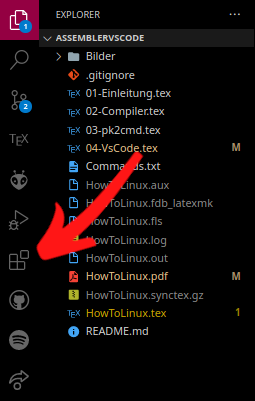
\includegraphics[scale=0.5]{WoExtensions.png} & \hspace{2cm} 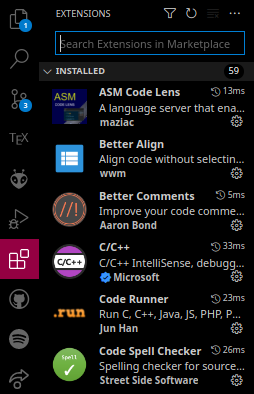
\includegraphics[scale=0.5]{Extensions.png}
    \end{tabular}
\end{center}
\begin{itemize}
    \item \enquote{Code Runner}\\
    Diese Extension macht uns möglich die Terminal-Befehle die in den vorherigen Kapitel erklärt habe über ein paar Klicks auszuführen.
    \begin{center}
        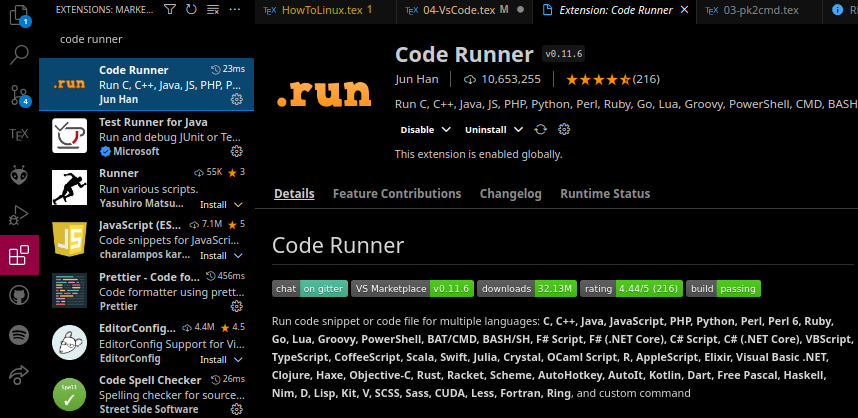
\includegraphics[scale=0.5]{codeRunner.png}
    \end{center}
    \item \enquote{ASM Code Lens}\\
    Diese Extension ist für das Syntax-Highlighting und den Language-Support verantwortlich. Damit lassen sich {\ttfamily .asm}-Files als \enquote{Assembler file} erkennen lassen. Weiterhin hat sie noch ein paar nützliche Feature wie Referenzen.
    \begin{center}
        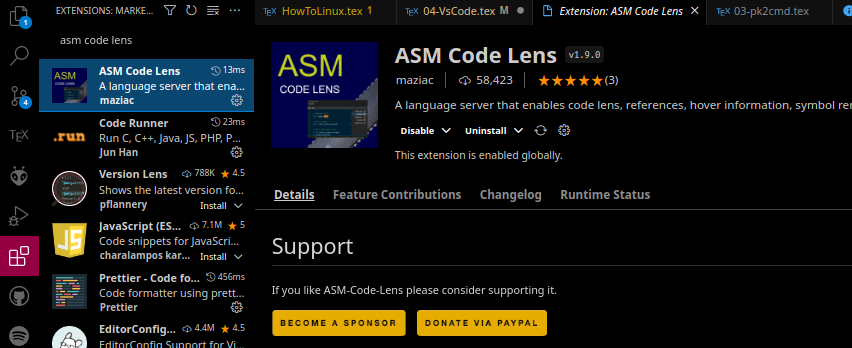
\includegraphics[scale=0.5]{asmCodeLens.png}
    \end{center}
\end{itemize}
\newpage
\subsection{Einstellungen}
Nun wollen wir VS Code nur sagen, was es zu tun hat. Dies kann man entweder in einer GUI in den Einstellungen machen oder in der {\ttfamily settings.json}. Ich zeige den zweiten Weg, da dieser einfacher ist zum ausführen.
\begin{itemize}
    \item[1)] Führen Sie die Tastenkombination \textbf{STRG+SHIFT+P} aus oder \textbf{View -> Command Palette} in der Menüleiste. Es sollte sich nun oben eine Suche aufgemacht haben. Dort geben sie \enquote{settings} ein und wählen die Option \enquote{Preferences: Open Settings (JSON)} auch nochmal gezeigt in der Abbildung.
    \begin{center}
        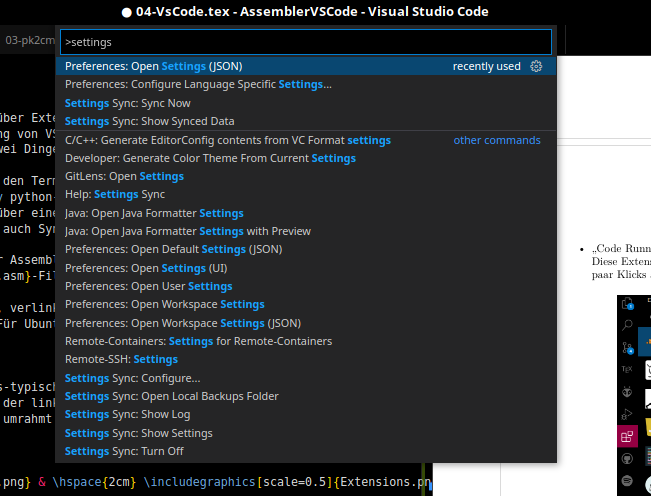
\includegraphics[scale=0.45]{commandPalette.png}
    \end{center}
    \item[2)] In diese Datei fügen sie folgende Code-Zeilen innerhalb der geschweiften Klammern ein (Ich habe in Kommentaren gekennzeichnet mit // reingeschrieben was welche Zeile macht)
\begin{lstlisting}[language=json]
// Sagt VS Code als was er .asm-Files und .INC-Files behandeln soll
"files.associations": {
    "*.asm": "asm-collection",
    "*.INC": "asm-collection"
},

// Code Runner
// Play-Button zum Ausfuehren des Codes in TitleMenu
"code-runner.showRunIconInEditorTitleMenu": true,
// Fuehrt Code in Terminal aus
"code-runner.runInTerminal": true,
// Befehle um .asm-File oder .hex-File auszufuehren mit dem PIC16F84A als Standard PIC
"code-runner.executorMap": {
    "asm-collection": "cd $dir && gpasm $fileNameWithoutExt.asm &&  pk2cmd -A5 -PPIC16F84A -F $fileNameWithoutExt.hex -M -T -R && cd $workspaceRoot",
    "hex": "cd $dir && pk2cmd -A5 -PPIC16F84A -F $fileNameWithoutExt.hex -M -T -R"
},
\end{lstlisting}
    \item[3)] Save mit \textbf{STRG+S}
\end{itemize}

\subsection{Erstes .asm-File ausführen}
Als letzten Punkt in dieser Anleitung zeige ich Ihnen wie Sie nun ein {\ttfamily .asm}-File ausführen können. Däfur drücken sie einfach \textbf{STRG+N} in VS Code. Es soll sich ein Tab aufgemacht haben mit dem Namen \enquote{Untitled-1}. In die frei Fläche fügen sie den Code \href{https://github.com/ManeLippert/AssemblerVSCode/blob/master/lauf.asm}{\ttfamily lauf.asm} den ich unten aufführe. Achten Sie auf die Formatierung!
\begin{lstlisting}[language={[x86masm]Assembler}]
;Von Reinhard Richter aus dem Kurs Prozessrechner und Elektronik

    processor	PIC16F84A
    include	p16f84a.inc

;Configurationword*************************************************************
    __CONFIG _CP_OFF & _XT_OSC & _WDT_OFF & _PWRTE_ON ;config: 0x3ff1

;INITIALISIERUNG***************************************************************
 org 0x000	;schreibe den naechsten Befehl an die Speicherstelle 0x000

        bsf	STATUS,RP0		;BANK1
        clrf	TRISA			;PORTA als AUSGANG
        clrf	TRISB			;PORTB als AUSGANG
        bcf	OPTION_REG,PSA		;Prescaler auf TMR0
        bsf	OPTION_REG,PS0		;
        bsf	OPTION_REG,PS1		;Prescaler auf 1:256
        bsf	OPTION_REG,PS2		;
        bcf	OPTION_REG,T0CS		;Internal Clock
        bcf	STATUS,RP0		;BANK0
        clrf	PORTA			;PORTA loeschen
        clrf	PORTB			;PORTB loeschen
        movlw	0x01			;00000001 in W
        movwf	0x0C			;lade W in Register 0x0C
        bcf	STATUS, C		;loesche das Carry-Bit

;HAUPTPROGRAMM*****************************************************************
MAIN
        movf	0x0C,W			;Lade den Inhalt von 0x0C nach W
        movwf	PORTA			;Kopiere W nach PORTA
        movwf	PORTB			;Kopiere W nach PORTB
        call	delay			;warte etwas
        rlf	0x0C,f			;Rotiere 0x0C nach links
        goto MAIN			;Schleife

;Delayschleife*****************************************************************
delay
        clrf	TMR0			;loesche TMR0
        bcf	INTCON,T0IF		;TMR0 overflow interrupt flag loeschen

delay_loop
        btfss	INTCON,T0IF		;springe wenn T0IF gesetzt
        goto	delay_loop			
        return

end
\end{lstlisting}
Speichern Sie den Code mit \textbf{STRG+S} und geben Sie ihm den Namen {\ttfamily lauf.asm}. Wenn alles geklappt sollte es bei Ihnen aussehen wie unten in der Abbildung. Wichtig ist dabei, dass unten rechts in der Status-Leiste (Bei mir rote Leiste) \enquote{Assembler file} steht. Wenn dies der Fall ist können Sie das PICkit 2 mit dem Microchip anschließen und oben in der rechten Ecke den grauen Play-Button drücken um den Code ausführen zu lassen. 
\begin{center}
    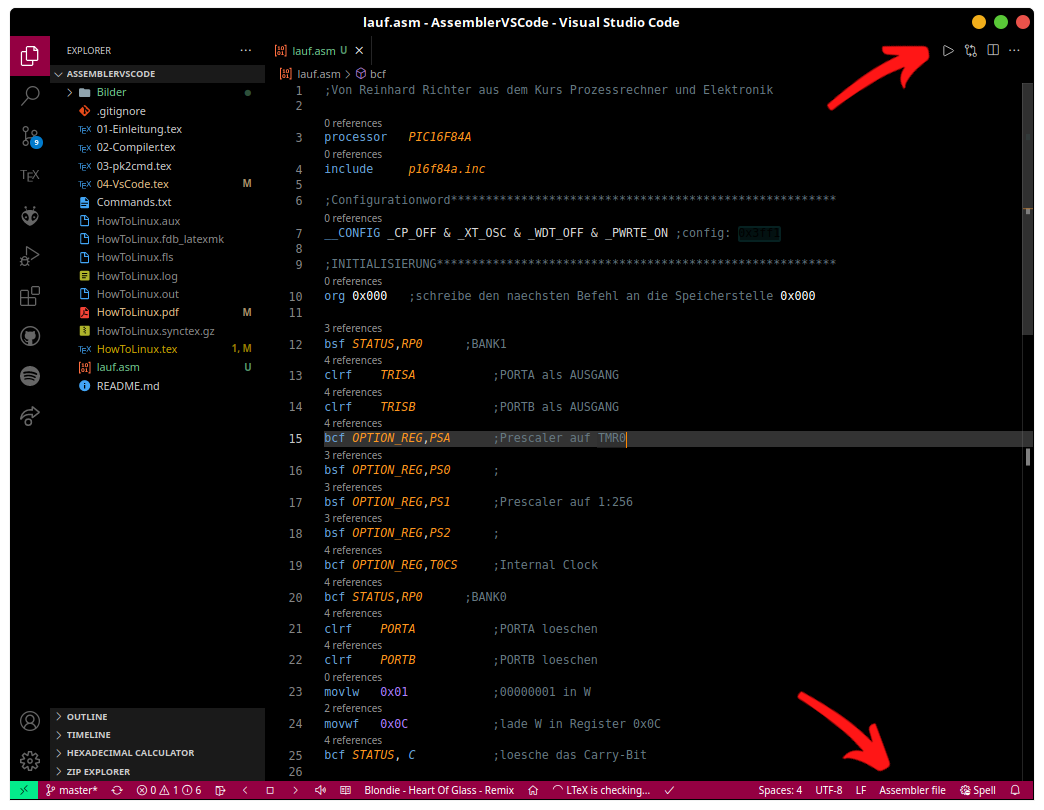
\includegraphics[scale=0.45]{lauf_overview_arrow.png}
\end{center}
Nach dem Drücken des grauen Play-Button sollte sich ein Terminal aufmachen, indem der Code, wie zuvor in CodeRunner spezifiziert wurde, ausgeführt wird. Der Output sollte am Ende dann so aussehen:
\begin{lstlisting}[language=bash]
                            Device Type: PIC16F84A

                            Program Succeeded.

                            Operation Succeeded 
\end{lstlisting}
Wenn alles geklappt hat, sollte dann sollten die LEDs in ein Lauflicht (Takt für Takt leuchtet eine andere LED auf) erzeugt worden sein. Damit sind Sie auch bereit absofort Assembler-Code in VS Code zu schreiben.